\section{Background and Motivation}
\label{sec:motivation}

\subsection{Distributed Vector Search and the Scaling Trap}
\label{subsec:background}

\noindent\textbf{Graph-based ANN search.} Vector similarity search is a foundational primitive for modern AI applications, including Retrieval-Augmented Generation (RAG) and large-scale recommendation systems. To process massive datasets efficiently, Approximate Nearest Neighbor (ANN) search is universally adopted. Among existing techniques, graph-based indexes (e.g., HNSW~\cite{malkov2018efficient}) have emerged as the industry standard by offering an optimal Pareto frontier of query latency and recall. These indexes represent vectors as nodes and connect spatially adjacent vectors via edges. Query execution relies on greedy routing: starting from a predefined entry node, the algorithm iteratively traverses edges to nodes progressively closer to the query vector. Consequently, the efficiency and accuracy of the search are fundamentally dictated by the topological connectivity of the graph, achieving a logarithmic search complexity of $\mathcal{O}(\log N)$.

\noindent\textbf{Scatter-gather architecture.} As datasets scale to billions of vectors, the memory footprint of the graph index quickly exceeds single-machine capacities. To scale out, modern distributed vector databases (e.g., Milvus, Qdrant, and Pinecone) predominantly adopt a \textit{scatter-gather} architecture. The global high-dimensional dataset is horizontally partitioned (sharded) across $P$ workers. Each worker independently constructs and maintains a disjoint local graph index over its assigned subset. When a client issues a top-$k$ search request, distributed execution proceeds through a three-stage pipeline:
\begin{enumerate}[leftmargin=*, topsep=2pt, itemsep=0pt, parsep=0pt]
    \item \textit{Routing:} The coordinator evaluates a routing policy to determine the subset of partitions (i.e., the \textit{fan-out} $f \le P$) that should process the query.
    \item \textit{Local search:} The selected workers concurrently execute the graph-based ANN search on their local indexes, retrieving their local top-$k$ candidates.
    \item \textit{Aggregation:} The workers return their partial results to the coordinator, which merges and globally sorts them to yield the final top-$k$.
\end{enumerate}

\noindent\textbf{The $\mathcal{O}(\log N)$ scaling trap.} By default, systems ensure perfect load balancing by randomly or hash-partitioning vectors, which destroys data locality. Consequently, the routing policy degenerates to \textit{broadcast} (fan-out $f = P$), sending every query to all shards to maintain high recall.

While perfectly load-balanced, broadcasting triggers a severe scalability bottleneck due to the logarithmic scaling property of graph-based search. Horizontally partitioning a dataset of $N$ vectors across $P$ machines reduces the local dataset size to $N/P$. Consequently, the local search time becomes proportional to $\mathcal{O}(\log(N/P)) = \mathcal{O}(\log N - \log P)$. Because the number of machines $P$ (e.g., tens or hundreds) is orders of magnitude smaller than the dataset size $N$ (e.g., billions), the $\log P$ term is mathematically negligible. 

For instance, splitting a billion-scale dataset ($N = 10^9$) across 16 machines ($P = 16$) reduces the theoretical search depth from $\log_2(10^9) \approx 30$ to $\log_2(10^9/16) \approx 26$. This means a $16\times$ increase in hardware resources yields a mere 13\% reduction in local traversal steps for any individual worker.

The convergence of broadcast routing and this scaling trap triggers a massive explosion in redundant computation. The aggregate CPU work performed by the cluster per query scales to $P \times \mathcal{O}(\log(N/P))$---roughly $P$ times the computational cost of searching the unpartitioned global graph. As the cluster scales out, this redundant work rapidly outpaces the addition of raw computational capacity, causing query throughput to stagnate.

\subsection{Motivation 1: Fan-out Reduction as the First-Order Lever}
\label{subsec:motivation_fanout}

To unlock true horizontal scalability, a distributed vector database must abandon broadcast and route queries only to a small subset of relevant shards (i.e., achieving $f \ll P$). Because the total computational work is dominated by the number of shards probed, reducing fan-out serves as the first-order lever for increasing system throughput. 

The industry's intuitive solution to reduce fan-out is \textit{geometric partitioning} (e.g., $K$-means clustering). During ingestion, the vector space is partitioned into $P$ geometric clusters, and vectors are assigned to shards based on their nearest centroid. During query execution, the coordinator computes the distance between the query and all $P$ centroids, routing the request only to the top-$nprobe$ nearest shards.

Our empirical measurements confirm the immense potential of fan-out reduction. We evaluated matched-recall query throughput (QPS) on a 46-shard cluster using the SIFT-1M dataset. Compared to the hash-based broadcast baseline (fan-out $f=46$), introducing a simple $K$-means geometric router (probing only $f \approx 11$ shards) increased the QPS by \textbf{3.4$\times$} at a strict Recall@10 target of 0.99. This confirms that regardless of the specific routing algorithm, aggressively pruning the fan-out is a mandatory prerequisite for distributed efficiency.

\subsection{Motivation 2: The Failure of Geometric Routing on Hard Workloads}
\label{subsec:motivation_failure}

Geometric routing works exceptionally well on ``easy'' workloads---datasets that are uniformly distributed and rely on Euclidean distance (e.g., SIFT). In such spaces, the geometric distance between a query and a cluster centroid perfectly correlates with the actual graph traversal path. As shown in our SIFT-1M experiments, the $K$-means centroid router achieves performance nearly identical to an optimal topology-aware router (a marginal 1.08$\times$ difference), proving that geometric partitioning is sufficient for simple distributions.

However, real-world AI workloads typically involve high-dimensional, highly skewed distributions and rely on angular or cosine distances (e.g., text embeddings, GloVe). On these ``hard'' workloads, geometric partitioning suffers from a fundamental flaw: the \textit{geometric-to-navigational gap}. 

In high-dimensional angular spaces, the geometric distance between a query and a partition's centroid no longer accurately predicts whether the true nearest neighbors reside in that partition. More importantly, it does not reflect the actual path a greedy graph search will take. A shard might geometrically overlap with the query, but lack the necessary topological connectivity (navigable edges) from its local entry points to the target vectors. 

Because centroid distance becomes a poor proxy for graph reachability, the coordinator frequently misroutes queries to suboptimal shards. To salvage the system's recall, the coordinator is forced to either drastically increase the fan-out ($nprobe$) or inflate the local search depth ($ef\_search$) within each shard. Both mitigations inject massive amounts of redundant computation, destroying the throughput gains achieved by partitioning.

Our measurements on the hard GloVe-200-angular dataset starkly highlight this failure. To achieve a Recall@10 of 0.90, the $K$-means centroid router is forced to consume massive internal search budgets (high $\Sigma ef$), yielding only 710 QPS. In contrast, a topology-aware routing mechanism (Orion, which we introduce next) achieves 1055 QPS at the exact same recall target---a \textbf{1.49$\times$} throughput advantage at equal storage capacity.

This is not an artifact of any single dataset. Table~\ref{tab:spectrum} sweeps four workloads spanning a spectrum of geometric difficulty---from SIFT (near-uniform image descriptors) through real OpenAI \texttt{text-embedding-ada-002} vectors and GloVe word vectors to Deep (learned CNN embeddings). The throughput advantage of topology-aware routing over the $K$-means centroid router tracks precisely how poorly geometric clustering captures the true-neighbor structure: a statistical tie on the near-uniform SIFT control, a solid $1.30\text{--}1.44\times$ on production OpenAI text embeddings, $1.49\times$ on GloVe, and $3.45\times$ on Deep---where the centroid router cannot even reach Recall $0.99$ at any fan-out. Every arm is served at \emph{equal storage} (a single copy per point, identical HNSW parameters), so the advantage comes from placement and routing rather than replication, and it is largest exactly in the neural-embedding regime that dominates modern RAG and recommendation workloads.

\begin{table}[t]
\centering
\small
\begin{tabular}{@{}llr@{}}
\toprule
Dataset (embedding) & Geometric character & Topo.\ vs.\ centroid \\
\midrule
SIFT-128 (image descriptors) & near-uniform (control) & $1.08\times$ (tie) \\
DBpedia-1536 (OpenAI ada-002) & moderately clusterable & $1.30\times$ \\
GloVe-200 (word vectors) & angular, skewed & $1.49\times$ \\
Deep-96 (learned CNN) & complex manifold & $3.45\times$ \\
\bottomrule
\end{tabular}
\caption{Matched-recall throughput advantage of topology-aware routing (Orion) over the $K$-means centroid router, across four datasets ordered by geometric difficulty. All arms are single-copy with identical HNSW parameters on a 46-shard cluster; the advantage grows as the embedding's neighbor structure departs from smooth geometric clusters. On Deep the centroid router additionally fails to reach Recall $0.99$ at any fan-out.}
\label{tab:spectrum}
\end{table}

This confirms that while geometric routing is a valid baseline, it fundamentally fails to unlock the full potential of distributed graph indices on complex, real-world vector distributions.

\subsection{Motivation 3: The Need for Topology-Aware Placement and Routing}
\label{subsec:motivation_topology}

To overcome the geometric-to-navigational gap, we must fundamentally rethink how vectors are partitioned and routed. Since ANN search on indices like HNSW is intrinsically a graph traversal process, the partitioning strategy should be dictated by the graph's topology, not the vector space's geometry. Vectors that are frequently co-accessed along the same greedy search paths should be co-located in the same shard. This perspective transforms the sharding problem from spatial clustering into a graph partitioning problem based on co-accessibility.

However, optimizing data placement is only half the solution. A fundamental principle of efficient distributed systems is \textit{offline-online symmetry}: the online routing mechanism must perfectly mirror the offline data placement logic. If data is partitioned based on graph topology, routing queries using geometric centroids will inevitably lead to mismatches. Instead, the coordinator requires a topological routing mechanism. By maintaining a global ``upper graph'' that acts as a macroscopic map of the distributed index, the coordinator can simulate the actual graph traversal. This allows it to accurately predict which shards contain the target vectors and, crucially, provide optimal entry points to seed the local search on those shards, further reducing the internal search work ($\Sigma ef$).

Furthermore, topological partitioning introduces a critical challenge: load skew. Geometric methods like $K$-means easily achieve \textit{size balance} (an equal number of vectors per shard). However, in graph-based search, node access frequencies are highly skewed; ``hub'' nodes are visited by almost every query, while isolated nodes are rarely touched. Consequently, size balance does not equate to \textit{load balance}. A robust partitioning algorithm must be \textit{capacity-constrained}, ensuring that the actual computational work (the number of query touches) is evenly distributed across the cluster, rather than just the storage footprint.

Recognizing these three requirements---topology-aware placement, symmetric graph-based routing, and capacity-constrained load balancing---we can now rigorously formalize the distributed vector search problem. By treating each query's traversal path as a hyperedge over the dataset, the goal of minimizing fan-out while maintaining load balance can be elegantly modeled mathematically. In the next section, we formalize this as a balanced minimum-cut problem on a workload hypergraph, laying the theoretical foundation for Orion.
% Orion --- Theory / Problem Formalization section (systems-paper style)
% ---------------------------------------------------------------------------
% Usage:
%   1) As an includable section, add to your preamble:
%        \usepackage{amsmath,amssymb,amsthm,booktabs}
%        \newtheorem{lemma}{Lemma}
%        \newtheorem{assumption}{Assumption}
%      then in the body:  % Orion --- Theory / Problem Formalization section (systems-paper style)
% ---------------------------------------------------------------------------
% Usage:
%   1) As an includable section, add to your preamble:
%        \usepackage{amsmath,amssymb,amsthm,booktabs}
%        \newtheorem{lemma}{Lemma}
%        \newtheorem{assumption}{Assumption}
%      then in the body:  % Orion --- Theory / Problem Formalization section (systems-paper style)
% ---------------------------------------------------------------------------
% Usage:
%   1) As an includable section, add to your preamble:
%        \usepackage{amsmath,amssymb,amsthm,booktabs}
%        \newtheorem{lemma}{Lemma}
%        \newtheorem{assumption}{Assumption}
%      then in the body:  % Orion --- Theory / Problem Formalization section (systems-paper style)
% ---------------------------------------------------------------------------
% Usage:
%   1) As an includable section, add to your preamble:
%        \usepackage{amsmath,amssymb,amsthm,booktabs}
%        \newtheorem{lemma}{Lemma}
%        \newtheorem{assumption}{Assumption}
%      then in the body:  \input{theory_section}
%   2) To compile this file standalone, uncomment the STANDALONE block below.
%
% Note: written in English per systems-venue convention (OSDI/NSDI/SOSP/VLDB/ATC).
% ---------------------------------------------------------------------------

% ------------------------- STANDALONE (uncomment) --------------------------
% \documentclass[11pt]{article}
% \usepackage[margin=1in]{geometry}
% \usepackage{amsmath,amssymb,amsthm,booktabs}
% \newtheorem{lemma}{Lemma}
% \newtheorem{assumption}{Assumption}
% \newtheorem{definition}{Definition}
% \begin{document}
% ---------------------------------------------------------------------------

\section{Sharding as Balanced Fan-out Minimization}
\label{sec:theory}

\paragraph{The sharding problem (mechanism-independent).}
We first state the problem without reference to any index structure. Let
$X=\{x_1,\dots,x_N\}$ be the dataset, $q\sim Q$ a query drawn from the workload,
and $\mathrm{NN}_k(q)\subseteq X$ its true $k$ nearest neighbors under the target
metric; $R$ denotes the target recall, i.e.\ we require Recall@$k\ge R$. A
sharding is an assignment $\sigma:X\to\{1,\dots,P\}$; \emph{replication}, which
lets a point occupy several shards, is a relaxation we treat at the end of this
section. To return the true neighbors, a
query must touch every shard that holds one of them, so its \emph{required
fan-out} is
\[
\mathrm{fanout}^\star_\sigma(q)=\bigl|\{\sigma(x):x\in\mathrm{NN}_k(q)\}\bigr|.
\]
This quantity depends only on the data, the workload, and the assignment---not on
how any system routes. At fixed recall the per-query server work is
$\sum_{s\,\text{probed}}\Theta(\mathrm{ef}_s\log|\text{shard}|)$, so with one shard
per core the throughput at saturation scales as
$P/\bigl(\mathbb{E}_q[\mathrm{fanout}]\cdot\rho\cdot\bar c\bigr)$, where $\rho$ is
the \emph{load skew} (busiest-over-mean per-shard query load) and $\bar c$ the
mean per-shard search cost (\S\ref{sec:motivation}, claim~C1). Fan-out is the
first-order term---it fixes the aggregate work---so we take it as the objective;
the load skew $\rho$ and the per-shard search strengths $\mathrm{ef}_s$ are
second-order factors that the same mechanism also controls (developed below and
measured in \S\ref{sec:eval}). The first-order sharding problem is
\begin{equation}
\label{eq:objective}
\min_{\sigma}\ \mathbb{E}_{q}\!\left[\mathrm{fanout}^\star_\sigma(q)\right]
\quad\text{s.t.}\quad
(1-\varepsilon)\tfrac{N}{P}\le |\sigma^{-1}(i)| \le (1+\varepsilon)\tfrac{N}{P}\ \ \forall i .
\end{equation}
The band constrains shard \emph{size} $|\sigma^{-1}(i)|$, a tractable surrogate
for the per-shard query \emph{load} that actually caps throughput; on a graph
index the two diverge---equal-sized shards can draw unequal traffic---so we
enforce size balance offline and report the residual load skew $\rho$ as a
separate diagnostic rather than fold it into~\eqref{eq:objective}.
\eqref{eq:objective} is an instance of a classical combinatorial problem, which
lets us reuse its known hardness and algorithms. A query's neighbor set
$\mathrm{NN}_k(q)$ ties together up to $k$ points that must be retrieved together,
a relation an ordinary (two-endpoint) edge cannot express. We therefore model the
workload as a \emph{hypergraph} $H=(X,\{e_q\}_q)$ whose vertices are the data
points and whose \emph{hyperedges} $e_q=\mathrm{NN}_k(q)$ each span all neighbors
of one query, with weight $c(e)=\Pr_q[\mathrm{NN}_k(q)=e]$. For an assignment
$\sigma$, let $\lambda(e)=|\{\sigma(x):x\in e\}|$ be the number of distinct shards
a hyperedge spans; by construction this is exactly the query's fan-out,
$\lambda(e_q)=\mathrm{fanout}^\star_\sigma(q)$. Hypergraph partitioning
conventionally minimizes the \emph{connectivity} (or ``$\lambda\!-\!1$'') metric
$\sum_e c(e)\,(\lambda(e)-1)$, i.e.\ how many \emph{extra} shards each hyperedge
reaches beyond its first---the standard measure of cross-partition communication.
Since $\sum_e c(e)=1$, this metric equals
$\mathbb{E}_q[\mathrm{fanout}^\star_\sigma(q)]-1$, so it has the \emph{same
minimizer} as~\eqref{eq:objective}: minimizing expected fan-out \emph{is}
minimizing the $\lambda\!-\!1$ objective, and the balance band is the standard
$(1{+}\varepsilon)$ balance constraint. Hence~\eqref{eq:objective} is a
$(P,1{+}\varepsilon)$-balanced minimum-connectivity hypergraph partitioning
instance ($P$ parts, within a $(1{+}\varepsilon)$ balance band)---the problem
solved by tools such as hMETIS and KaHyPar~\cite{metis,kahypar}. (For a target
$R<1$, $\mathrm{NN}_k(q)$ is replaced by a recall-$R$ sufficient subset, which can
only lower fan-out; the full-neighbor version above is the conservative
reference.) Even for fixed
$P$ with the relaxed balance constraint this problem is NP-hard, and
inapproximable under strictly equal parts~\cite{andreev2006}, which is why Orion
optimizes a computable surrogate rather than~\eqref{eq:objective} itself, as the
next paragraphs develop.

\paragraph{Why the problem cannot be optimized directly.}
Two gaps prevent solving~\eqref{eq:objective} as stated. \emph{Offline}, the
hyperedges $\mathrm{NN}_k(q)$ are query-specific and the workload is not known in
advance; materializing ground-truth neighbors for a representative query sample
at scale is expensive, so the partitioner needs a computable, query-independent
proxy for which points are \emph{co-relevant}. \emph{Online}, $\mathrm{NN}_k(q)$
is precisely the unknown the query is trying to find, so a router must estimate
which shards hold the neighbors without an exhaustive scan. Any practical system
must supply a mechanism for both; the navigation graph is Orion's, and it is a
component of the \emph{solution}, not a premise of the problem.

\paragraph{Orion's navigation-graph instantiation.}
Orion introduces a single frozen \emph{upper navigation graph} $G=(V,E,w)$, where
$V$ are upper navigation points and $E$ is its directed adjacency. We define the
\emph{navigation traffic}
\begin{equation}
\label{eq:traffic}
w(u,v)=\mathbb{E}_{q}\bigl[\,\#\{\text{times $q$'s traversal explores }(u,v)\}\,\bigr],
\end{equation}
the expected number of times, \emph{per query}, that the frozen navigator
evaluates $v$ as a neighbor of an expanded node $u$. This is exactly the
search-induced evidence Orion already materializes as attachment votes; it is not
raw geometric distance. Its working hypothesis (\emph{search-induced topology}) is
that $w$ is a computable proxy for co-relevance: points reached together during
navigation tend to fall in a common query's neighbor set. This closes both gaps
with one artifact.

\emph{Offline}, Orion replaces the intractable hypergraph
objective~\eqref{eq:objective} by a tractable \emph{graph} surrogate on $G$.
For an upper membership $\pi:V\to\{1,\dots,P\}$, the
\emph{navigation-weighted cut}
$\sum_{(u,v):\pi(u)\neq\pi(v)}w(u,v)$ sums the traffic on edges whose endpoints
lie in different shards---intuitively, how often navigation would have to leave
one shard for another. Minimizing it under the same balance band is the standard
approach taken by multilevel partitioners~\cite{metis,kahypar}, and Orion
implements it in three classical stages:
\begin{enumerate}
\item \emph{Initialization.} A geometric $k$-means clustering of the upper
  vectors into $P$ shards yields a cheap first assignment that ignores graph
  structure but is already roughly balanced.
\item \emph{Move-based refinement.} Following the Kernighan--Lin /
  Fiduccia--Mattheyses family~\cite{kl1970,fm1982}, Orion repeatedly considers
  moving a single upper point from its current shard to another. A move's
  \emph{gain} is the change in weighted cut (plus a topology vote from
  navigation evidence); a move is accepted only if its gain is nonnegative (or
  repairs a balance violation) and the target shard still has spare capacity.
  Sequential, capacity-aware acceptance avoids the classic collapse where many
  nodes race into the same underfull shard in one synchronous round.
\item \emph{Balance repair.} If some shards still violate the
  $(1{\pm}\varepsilon)$ band after refinement, Orion solves a small
  \emph{transportation} (min-cost flow) problem: overloaded shards are sources,
  underloaded shards are sinks, and admissible arcs are those justified by
  navigation evidence. Shipping one unit of flow along an arc corresponds to
  reassigning one point (or a group of points); the optimum restores balance at
  minimal disruption to the cut.
\end{enumerate}
All three stages read only the frozen upper graph, so the offline cost stays
near-linear and the result is checksum-reproducible.

\emph{Online}, serving is two-stage: a global traversal of $G$ selects shards and
per-shard entry points $\mathrm{EP}(q)\subseteq\mathrm{Vis}(q)$ (the estimator of
the neighbor-bearing shards), after which each selected shard runs an
\emph{independent} local search whose \emph{strength} scales with the same
evidence: a shard receiving more of $q$'s entry points is searched at a larger
$\mathrm{ef}_s=\mathrm{ef}_0+\gamma\,|\mathrm{EP}(q)\cap\pi^{-1}(s)|$. The
navigation signal thus governs both \emph{which} shards are probed (the fan-out)
and \emph{how hard} each is searched (the effort budget $\sum_s\mathrm{ef}_s$),
concentrating work on the shards navigation implicates. The \emph{realized}
fan-out is
$\mathrm{fanout}^\pi(q)=|\{\pi(v):v\in\mathrm{EP}(q)\}|$; base-layer placement
follows $\pi$ under the same balance band.

\paragraph{A mechanism-side bound and a recall assumption.}
Two claims connect Orion's mechanism back to the problem. First, the offline
objective it actually optimizes---the navigation-weighted cut---upper-bounds the
\emph{realized} online fan-out (Lemma~\ref{lem:fanout}). Second, minimizing that
realized fan-out is meaningful only if the router still returns the neighbors,
which we state as an explicit, empirically testable assumption
(Assumption~\ref{ass:recall}) rather than fold into the definitions.

\begin{lemma}[Realized fan-out is dominated by the weighted cut]
\label{lem:fanout}
Let $\mathrm{cut}(\pi)=\{(u,v)\in E:\pi(u)\neq\pi(v)\}$ and let $w$ be the
navigation traffic of~\eqref{eq:traffic}. Then
\[
\mathbb{E}_{q}\!\left[\mathrm{fanout}^\pi(q)\right]
\ \le\ 1+\!\!\sum_{(u,v)\in\mathrm{cut}(\pi)}\!\! w(u,v).
\]
\end{lemma}

\begin{proof}
Fix a query $q$, let $\mathrm{Vis}(q)$ be the set of nodes its upper traversal
expands, and let $T(q)\subseteq E$ be the set of edges the traversal explores.
Best-first search discovers a node only by exploring an edge out of an
already-expanded node, so $(\mathrm{Vis}(q),T(q))$ is \emph{connected}: it
contains a spanning tree rooted at the entry node. We stress that we do not
assume the expansion order forms a walk in $G$---consecutive expanded nodes need
not be adjacent, since candidates are popped from a priority queue.

Let $m=\bigl|\{\pi(v):v\in\mathrm{Vis}(q)\}\bigr|$ be the number of shards the
visited set spans, and contract each shard's portion of $\mathrm{Vis}(q)$ into a
single supernode. The contracted multigraph has $m$ supernodes and inherits
connectivity, hence carries at least $m-1$ edges; each of them is an explored
edge whose endpoints lie in different shards. Therefore
\[
m\ \le\ 1+\bigl|\{(u,v)\in T(q):\pi(u)\neq\pi(v)\}\bigr|.
\]
Entry points are selected only among expanded nodes, so
$\mathrm{EP}(q)\subseteq\mathrm{Vis}(q)$ and $\mathrm{fanout}^\pi(q)\le m$. Taking
expectations over $q$ and applying~\eqref{eq:traffic} edgewise,
$\mathbb{E}_q\bigl|\{(u,v)\in T(q):\pi(u)\neq\pi(v)\}\bigr|
=\sum_{(u,v)\in\mathrm{cut}(\pi)}w(u,v)$, which yields the claim.
\end{proof}

The bound is loose in two safe directions: fan-out counts only the shards of the
selected entry points, a subset of the visited shards, and a traversal that
repeatedly explores edges between the same two shards pays each time in the cut
but only once in fan-out. Thus the navigation-weighted cut is a
\emph{conservative} upper bound on realized fan-out, so optimizing it never
underestimates online cost.

A natural refinement of the same idea normalizes each shard's cut by its
\emph{volume} (total incident traffic)
$\mathrm{vol}(V_i)=\sum_{u\in V_i}\sum_{v}w(u,v)$, yielding the
\emph{conductance} (or normalized-cut) of the partition:
\[
\phi(\pi)=\sum_{i=1}^{P}\frac{\sum_{(u,v):\pi(u)=i,\pi(v)\neq i}w(u,v)}{\mathrm{vol}(V_i)}.
\]
Each summand is the probability that a random navigation step taken inside shard
$i$ immediately leaves it, and $\phi$ sums these escape probabilities over shards
(the normalized cut of Shi and Malik~\cite{shimalik2000}). Low conductance
therefore means every
shard is a \emph{metastable} region of the upper traversal---a set navigation
enters and then tends to stay in. Under this reading, the search-induced-topology hypothesis
simply says: shards that are metastable for navigation are the ones whose
interior points are co-relevant for the same queries, and are therefore the
right blocks for~\eqref{eq:objective}.

\begin{assumption}[Navigation preserves recall]
\label{ass:recall}
For target recall $R$, with high probability over $q\sim Q$ the shards selected by
the upper traversal, $\{\pi(v):v\in\mathrm{EP}(q)\}$, contain a recall-$R$
sufficient subset of $\mathrm{NN}_k(q)$.
\end{assumption}

Under Assumption~\ref{ass:recall}, Orion's router attains the target recall, so
its realized fan-out $\mathrm{fanout}^\pi$ is an \emph{achievable} cost for the
sharding problem, and by Lemma~\ref{lem:fanout} that cost is controlled by the
offline cut Orion minimizes. The required fan-out
$\mathrm{fanout}^\star_\sigma$ remains the mechanism-free reference against which
we report the residual gap; neither direction of comparison is automatic, since a
router targeting $R<1$ may deliberately skip a shard that holds a true neighbor.
The navigation graph thus links the mechanism-independent
objective to a computable surrogate \emph{without} being assumed in the problem
statement; Assumption~\ref{ass:recall} is what \S\ref{sec:eval} measures, and it
can fail---in which case the surrogate is simply a worse proxy, not a redefinition
of the problem.

\paragraph{From theory to mechanism.}
Table~\ref{tab:theory-map} maps each quantity in the formalization to the
concrete Orion mechanism and to the metric we report, so the design and the
evaluation can be read against the same objects.

One further design choice maps to a standard graph-partitioning relaxation.
So far $\sigma$ assigns each point to a single shard (\emph{edge-cut} style:
the cut is paid by edges that cross the boundary). Orion's
\emph{multi-assignment} instead lets a point occupy several shards, which is
the \emph{vertex-cut} (or overlapping) relaxation: a point that sits on a
search-relevant boundary is \emph{replicated} into the shards that navigation
evidence nominates. Replication lowers $\lambda$ for the hyperedges that
contain that point---the query no longer needs an extra hop to reach a copy---at
the cost of storing more physical copies. Formally, replication generalizes
$\sigma$ to $X\to 2^{\{1,\dots,P\}}$, the required fan-out becomes the smallest
number of shards \emph{covering} $\mathrm{NN}_k(q)$, and shard load is measured in
physical copies: with $M=\sum_{x\in X}|\sigma(x)|$ total copies, the balance band
in~\eqref{eq:objective} becomes $(1\pm\varepsilon)M/P$. The expansion ratio $M/N$
is the price of this relaxation, and is reported alongside fan-out so the
trade-off is explicit.

\begin{table}[t]
\centering
\small
\begin{tabular}{@{}lll@{}}
\toprule
Theoretical quantity & Orion mechanism & Reported metric \\
\midrule
Weighted cut / conductance & CCNB offline objective & cross-shard traffic \\
$\mathbb{E}[\mathrm{fanout}^\pi]$ (Lem.~\ref{lem:fanout}) & selective routing & visited logical shards \\
Balance band $(1{\pm}\varepsilon)$ & fixed-$P$ balancing & max/mean, CV \\
Load skew $\rho$ (2nd order) & size balance as proxy & max/mean query load \\
Per-shard strength $\mathrm{ef}_s$ (2nd order) & effort-scaled local search & within-shard work \\
Vertex-cut replication & multi-assignment & expansion ratio \\
\bottomrule
\end{tabular}
\caption{Correspondence between the partitioning formalization
(\S\ref{sec:theory}) and Orion's system mechanisms and measured quantities.}
\label{tab:theory-map}
\end{table}

We do not claim an approximation guarantee; instead, \S\ref{sec:eval}
empirically validates Lemma~\ref{lem:fanout} by correlating the offline
navigation-weighted cut (and conductance) with measured fan-out and end-to-end
QPS across $P\in\{4,8,16,32\}$, and tests Assumption~\ref{ass:recall} by checking
that the selected shards cover the true neighbors at the target recall. It also
quantifies the two second-order factors: the residual load skew $\rho$ that
survives size balancing, and the within-shard work that the effort-scaled
$\mathrm{ef}_s$ saves against a uniform-$\mathrm{ef}$ baseline at matched recall.

% ------------------------- STANDALONE (uncomment) --------------------------
% \end{document}
% ---------------------------------------------------------------------------

%   2) To compile this file standalone, uncomment the STANDALONE block below.
%
% Note: written in English per systems-venue convention (OSDI/NSDI/SOSP/VLDB/ATC).
% ---------------------------------------------------------------------------

% ------------------------- STANDALONE (uncomment) --------------------------
% \documentclass[11pt]{article}
% \usepackage[margin=1in]{geometry}
% \usepackage{amsmath,amssymb,amsthm,booktabs}
% \newtheorem{lemma}{Lemma}
% \newtheorem{assumption}{Assumption}
% \newtheorem{definition}{Definition}
% \begin{document}
% ---------------------------------------------------------------------------

\section{Sharding as Balanced Fan-out Minimization}
\label{sec:theory}

\paragraph{The sharding problem (mechanism-independent).}
We first state the problem without reference to any index structure. Let
$X=\{x_1,\dots,x_N\}$ be the dataset, $q\sim Q$ a query drawn from the workload,
and $\mathrm{NN}_k(q)\subseteq X$ its true $k$ nearest neighbors under the target
metric; $R$ denotes the target recall, i.e.\ we require Recall@$k\ge R$. A
sharding is an assignment $\sigma:X\to\{1,\dots,P\}$; \emph{replication}, which
lets a point occupy several shards, is a relaxation we treat at the end of this
section. To return the true neighbors, a
query must touch every shard that holds one of them, so its \emph{required
fan-out} is
\[
\mathrm{fanout}^\star_\sigma(q)=\bigl|\{\sigma(x):x\in\mathrm{NN}_k(q)\}\bigr|.
\]
This quantity depends only on the data, the workload, and the assignment---not on
how any system routes. At fixed recall the per-query server work is
$\sum_{s\,\text{probed}}\Theta(\mathrm{ef}_s\log|\text{shard}|)$, so with one shard
per core the throughput at saturation scales as
$P/\bigl(\mathbb{E}_q[\mathrm{fanout}]\cdot\rho\cdot\bar c\bigr)$, where $\rho$ is
the \emph{load skew} (busiest-over-mean per-shard query load) and $\bar c$ the
mean per-shard search cost (\S\ref{sec:motivation}, claim~C1). Fan-out is the
first-order term---it fixes the aggregate work---so we take it as the objective;
the load skew $\rho$ and the per-shard search strengths $\mathrm{ef}_s$ are
second-order factors that the same mechanism also controls (developed below and
measured in \S\ref{sec:eval}). The first-order sharding problem is
\begin{equation}
\label{eq:objective}
\min_{\sigma}\ \mathbb{E}_{q}\!\left[\mathrm{fanout}^\star_\sigma(q)\right]
\quad\text{s.t.}\quad
(1-\varepsilon)\tfrac{N}{P}\le |\sigma^{-1}(i)| \le (1+\varepsilon)\tfrac{N}{P}\ \ \forall i .
\end{equation}
The band constrains shard \emph{size} $|\sigma^{-1}(i)|$, a tractable surrogate
for the per-shard query \emph{load} that actually caps throughput; on a graph
index the two diverge---equal-sized shards can draw unequal traffic---so we
enforce size balance offline and report the residual load skew $\rho$ as a
separate diagnostic rather than fold it into~\eqref{eq:objective}.
\eqref{eq:objective} is an instance of a classical combinatorial problem, which
lets us reuse its known hardness and algorithms. A query's neighbor set
$\mathrm{NN}_k(q)$ ties together up to $k$ points that must be retrieved together,
a relation an ordinary (two-endpoint) edge cannot express. We therefore model the
workload as a \emph{hypergraph} $H=(X,\{e_q\}_q)$ whose vertices are the data
points and whose \emph{hyperedges} $e_q=\mathrm{NN}_k(q)$ each span all neighbors
of one query, with weight $c(e)=\Pr_q[\mathrm{NN}_k(q)=e]$. For an assignment
$\sigma$, let $\lambda(e)=|\{\sigma(x):x\in e\}|$ be the number of distinct shards
a hyperedge spans; by construction this is exactly the query's fan-out,
$\lambda(e_q)=\mathrm{fanout}^\star_\sigma(q)$. Hypergraph partitioning
conventionally minimizes the \emph{connectivity} (or ``$\lambda\!-\!1$'') metric
$\sum_e c(e)\,(\lambda(e)-1)$, i.e.\ how many \emph{extra} shards each hyperedge
reaches beyond its first---the standard measure of cross-partition communication.
Since $\sum_e c(e)=1$, this metric equals
$\mathbb{E}_q[\mathrm{fanout}^\star_\sigma(q)]-1$, so it has the \emph{same
minimizer} as~\eqref{eq:objective}: minimizing expected fan-out \emph{is}
minimizing the $\lambda\!-\!1$ objective, and the balance band is the standard
$(1{+}\varepsilon)$ balance constraint. Hence~\eqref{eq:objective} is a
$(P,1{+}\varepsilon)$-balanced minimum-connectivity hypergraph partitioning
instance ($P$ parts, within a $(1{+}\varepsilon)$ balance band)---the problem
solved by tools such as hMETIS and KaHyPar~\cite{metis,kahypar}. (For a target
$R<1$, $\mathrm{NN}_k(q)$ is replaced by a recall-$R$ sufficient subset, which can
only lower fan-out; the full-neighbor version above is the conservative
reference.) Even for fixed
$P$ with the relaxed balance constraint this problem is NP-hard, and
inapproximable under strictly equal parts~\cite{andreev2006}, which is why Orion
optimizes a computable surrogate rather than~\eqref{eq:objective} itself, as the
next paragraphs develop.

\paragraph{Why the problem cannot be optimized directly.}
Two gaps prevent solving~\eqref{eq:objective} as stated. \emph{Offline}, the
hyperedges $\mathrm{NN}_k(q)$ are query-specific and the workload is not known in
advance; materializing ground-truth neighbors for a representative query sample
at scale is expensive, so the partitioner needs a computable, query-independent
proxy for which points are \emph{co-relevant}. \emph{Online}, $\mathrm{NN}_k(q)$
is precisely the unknown the query is trying to find, so a router must estimate
which shards hold the neighbors without an exhaustive scan. Any practical system
must supply a mechanism for both; the navigation graph is Orion's, and it is a
component of the \emph{solution}, not a premise of the problem.

\paragraph{Orion's navigation-graph instantiation.}
Orion introduces a single frozen \emph{upper navigation graph} $G=(V,E,w)$, where
$V$ are upper navigation points and $E$ is its directed adjacency. We define the
\emph{navigation traffic}
\begin{equation}
\label{eq:traffic}
w(u,v)=\mathbb{E}_{q}\bigl[\,\#\{\text{times $q$'s traversal explores }(u,v)\}\,\bigr],
\end{equation}
the expected number of times, \emph{per query}, that the frozen navigator
evaluates $v$ as a neighbor of an expanded node $u$. This is exactly the
search-induced evidence Orion already materializes as attachment votes; it is not
raw geometric distance. Its working hypothesis (\emph{search-induced topology}) is
that $w$ is a computable proxy for co-relevance: points reached together during
navigation tend to fall in a common query's neighbor set. This closes both gaps
with one artifact.

\emph{Offline}, Orion replaces the intractable hypergraph
objective~\eqref{eq:objective} by a tractable \emph{graph} surrogate on $G$.
For an upper membership $\pi:V\to\{1,\dots,P\}$, the
\emph{navigation-weighted cut}
$\sum_{(u,v):\pi(u)\neq\pi(v)}w(u,v)$ sums the traffic on edges whose endpoints
lie in different shards---intuitively, how often navigation would have to leave
one shard for another. Minimizing it under the same balance band is the standard
approach taken by multilevel partitioners~\cite{metis,kahypar}, and Orion
implements it in three classical stages:
\begin{enumerate}
\item \emph{Initialization.} A geometric $k$-means clustering of the upper
  vectors into $P$ shards yields a cheap first assignment that ignores graph
  structure but is already roughly balanced.
\item \emph{Move-based refinement.} Following the Kernighan--Lin /
  Fiduccia--Mattheyses family~\cite{kl1970,fm1982}, Orion repeatedly considers
  moving a single upper point from its current shard to another. A move's
  \emph{gain} is the change in weighted cut (plus a topology vote from
  navigation evidence); a move is accepted only if its gain is nonnegative (or
  repairs a balance violation) and the target shard still has spare capacity.
  Sequential, capacity-aware acceptance avoids the classic collapse where many
  nodes race into the same underfull shard in one synchronous round.
\item \emph{Balance repair.} If some shards still violate the
  $(1{\pm}\varepsilon)$ band after refinement, Orion solves a small
  \emph{transportation} (min-cost flow) problem: overloaded shards are sources,
  underloaded shards are sinks, and admissible arcs are those justified by
  navigation evidence. Shipping one unit of flow along an arc corresponds to
  reassigning one point (or a group of points); the optimum restores balance at
  minimal disruption to the cut.
\end{enumerate}
All three stages read only the frozen upper graph, so the offline cost stays
near-linear and the result is checksum-reproducible.

\emph{Online}, serving is two-stage: a global traversal of $G$ selects shards and
per-shard entry points $\mathrm{EP}(q)\subseteq\mathrm{Vis}(q)$ (the estimator of
the neighbor-bearing shards), after which each selected shard runs an
\emph{independent} local search whose \emph{strength} scales with the same
evidence: a shard receiving more of $q$'s entry points is searched at a larger
$\mathrm{ef}_s=\mathrm{ef}_0+\gamma\,|\mathrm{EP}(q)\cap\pi^{-1}(s)|$. The
navigation signal thus governs both \emph{which} shards are probed (the fan-out)
and \emph{how hard} each is searched (the effort budget $\sum_s\mathrm{ef}_s$),
concentrating work on the shards navigation implicates. The \emph{realized}
fan-out is
$\mathrm{fanout}^\pi(q)=|\{\pi(v):v\in\mathrm{EP}(q)\}|$; base-layer placement
follows $\pi$ under the same balance band.

\paragraph{A mechanism-side bound and a recall assumption.}
Two claims connect Orion's mechanism back to the problem. First, the offline
objective it actually optimizes---the navigation-weighted cut---upper-bounds the
\emph{realized} online fan-out (Lemma~\ref{lem:fanout}). Second, minimizing that
realized fan-out is meaningful only if the router still returns the neighbors,
which we state as an explicit, empirically testable assumption
(Assumption~\ref{ass:recall}) rather than fold into the definitions.

\begin{lemma}[Realized fan-out is dominated by the weighted cut]
\label{lem:fanout}
Let $\mathrm{cut}(\pi)=\{(u,v)\in E:\pi(u)\neq\pi(v)\}$ and let $w$ be the
navigation traffic of~\eqref{eq:traffic}. Then
\[
\mathbb{E}_{q}\!\left[\mathrm{fanout}^\pi(q)\right]
\ \le\ 1+\!\!\sum_{(u,v)\in\mathrm{cut}(\pi)}\!\! w(u,v).
\]
\end{lemma}

\begin{proof}
Fix a query $q$, let $\mathrm{Vis}(q)$ be the set of nodes its upper traversal
expands, and let $T(q)\subseteq E$ be the set of edges the traversal explores.
Best-first search discovers a node only by exploring an edge out of an
already-expanded node, so $(\mathrm{Vis}(q),T(q))$ is \emph{connected}: it
contains a spanning tree rooted at the entry node. We stress that we do not
assume the expansion order forms a walk in $G$---consecutive expanded nodes need
not be adjacent, since candidates are popped from a priority queue.

Let $m=\bigl|\{\pi(v):v\in\mathrm{Vis}(q)\}\bigr|$ be the number of shards the
visited set spans, and contract each shard's portion of $\mathrm{Vis}(q)$ into a
single supernode. The contracted multigraph has $m$ supernodes and inherits
connectivity, hence carries at least $m-1$ edges; each of them is an explored
edge whose endpoints lie in different shards. Therefore
\[
m\ \le\ 1+\bigl|\{(u,v)\in T(q):\pi(u)\neq\pi(v)\}\bigr|.
\]
Entry points are selected only among expanded nodes, so
$\mathrm{EP}(q)\subseteq\mathrm{Vis}(q)$ and $\mathrm{fanout}^\pi(q)\le m$. Taking
expectations over $q$ and applying~\eqref{eq:traffic} edgewise,
$\mathbb{E}_q\bigl|\{(u,v)\in T(q):\pi(u)\neq\pi(v)\}\bigr|
=\sum_{(u,v)\in\mathrm{cut}(\pi)}w(u,v)$, which yields the claim.
\end{proof}

The bound is loose in two safe directions: fan-out counts only the shards of the
selected entry points, a subset of the visited shards, and a traversal that
repeatedly explores edges between the same two shards pays each time in the cut
but only once in fan-out. Thus the navigation-weighted cut is a
\emph{conservative} upper bound on realized fan-out, so optimizing it never
underestimates online cost.

A natural refinement of the same idea normalizes each shard's cut by its
\emph{volume} (total incident traffic)
$\mathrm{vol}(V_i)=\sum_{u\in V_i}\sum_{v}w(u,v)$, yielding the
\emph{conductance} (or normalized-cut) of the partition:
\[
\phi(\pi)=\sum_{i=1}^{P}\frac{\sum_{(u,v):\pi(u)=i,\pi(v)\neq i}w(u,v)}{\mathrm{vol}(V_i)}.
\]
Each summand is the probability that a random navigation step taken inside shard
$i$ immediately leaves it, and $\phi$ sums these escape probabilities over shards
(the normalized cut of Shi and Malik~\cite{shimalik2000}). Low conductance
therefore means every
shard is a \emph{metastable} region of the upper traversal---a set navigation
enters and then tends to stay in. Under this reading, the search-induced-topology hypothesis
simply says: shards that are metastable for navigation are the ones whose
interior points are co-relevant for the same queries, and are therefore the
right blocks for~\eqref{eq:objective}.

\begin{assumption}[Navigation preserves recall]
\label{ass:recall}
For target recall $R$, with high probability over $q\sim Q$ the shards selected by
the upper traversal, $\{\pi(v):v\in\mathrm{EP}(q)\}$, contain a recall-$R$
sufficient subset of $\mathrm{NN}_k(q)$.
\end{assumption}

Under Assumption~\ref{ass:recall}, Orion's router attains the target recall, so
its realized fan-out $\mathrm{fanout}^\pi$ is an \emph{achievable} cost for the
sharding problem, and by Lemma~\ref{lem:fanout} that cost is controlled by the
offline cut Orion minimizes. The required fan-out
$\mathrm{fanout}^\star_\sigma$ remains the mechanism-free reference against which
we report the residual gap; neither direction of comparison is automatic, since a
router targeting $R<1$ may deliberately skip a shard that holds a true neighbor.
The navigation graph thus links the mechanism-independent
objective to a computable surrogate \emph{without} being assumed in the problem
statement; Assumption~\ref{ass:recall} is what \S\ref{sec:eval} measures, and it
can fail---in which case the surrogate is simply a worse proxy, not a redefinition
of the problem.

\paragraph{From theory to mechanism.}
Table~\ref{tab:theory-map} maps each quantity in the formalization to the
concrete Orion mechanism and to the metric we report, so the design and the
evaluation can be read against the same objects.

One further design choice maps to a standard graph-partitioning relaxation.
So far $\sigma$ assigns each point to a single shard (\emph{edge-cut} style:
the cut is paid by edges that cross the boundary). Orion's
\emph{multi-assignment} instead lets a point occupy several shards, which is
the \emph{vertex-cut} (or overlapping) relaxation: a point that sits on a
search-relevant boundary is \emph{replicated} into the shards that navigation
evidence nominates. Replication lowers $\lambda$ for the hyperedges that
contain that point---the query no longer needs an extra hop to reach a copy---at
the cost of storing more physical copies. Formally, replication generalizes
$\sigma$ to $X\to 2^{\{1,\dots,P\}}$, the required fan-out becomes the smallest
number of shards \emph{covering} $\mathrm{NN}_k(q)$, and shard load is measured in
physical copies: with $M=\sum_{x\in X}|\sigma(x)|$ total copies, the balance band
in~\eqref{eq:objective} becomes $(1\pm\varepsilon)M/P$. The expansion ratio $M/N$
is the price of this relaxation, and is reported alongside fan-out so the
trade-off is explicit.

\begin{table}[t]
\centering
\small
\begin{tabular}{@{}lll@{}}
\toprule
Theoretical quantity & Orion mechanism & Reported metric \\
\midrule
Weighted cut / conductance & CCNB offline objective & cross-shard traffic \\
$\mathbb{E}[\mathrm{fanout}^\pi]$ (Lem.~\ref{lem:fanout}) & selective routing & visited logical shards \\
Balance band $(1{\pm}\varepsilon)$ & fixed-$P$ balancing & max/mean, CV \\
Load skew $\rho$ (2nd order) & size balance as proxy & max/mean query load \\
Per-shard strength $\mathrm{ef}_s$ (2nd order) & effort-scaled local search & within-shard work \\
Vertex-cut replication & multi-assignment & expansion ratio \\
\bottomrule
\end{tabular}
\caption{Correspondence between the partitioning formalization
(\S\ref{sec:theory}) and Orion's system mechanisms and measured quantities.}
\label{tab:theory-map}
\end{table}

We do not claim an approximation guarantee; instead, \S\ref{sec:eval}
empirically validates Lemma~\ref{lem:fanout} by correlating the offline
navigation-weighted cut (and conductance) with measured fan-out and end-to-end
QPS across $P\in\{4,8,16,32\}$, and tests Assumption~\ref{ass:recall} by checking
that the selected shards cover the true neighbors at the target recall. It also
quantifies the two second-order factors: the residual load skew $\rho$ that
survives size balancing, and the within-shard work that the effort-scaled
$\mathrm{ef}_s$ saves against a uniform-$\mathrm{ef}$ baseline at matched recall.

% ------------------------- STANDALONE (uncomment) --------------------------
% \end{document}
% ---------------------------------------------------------------------------

%   2) To compile this file standalone, uncomment the STANDALONE block below.
%
% Note: written in English per systems-venue convention (OSDI/NSDI/SOSP/VLDB/ATC).
% ---------------------------------------------------------------------------

% ------------------------- STANDALONE (uncomment) --------------------------
% \documentclass[11pt]{article}
% \usepackage[margin=1in]{geometry}
% \usepackage{amsmath,amssymb,amsthm,booktabs}
% \newtheorem{lemma}{Lemma}
% \newtheorem{assumption}{Assumption}
% \newtheorem{definition}{Definition}
% \begin{document}
% ---------------------------------------------------------------------------

\section{Sharding as Balanced Fan-out Minimization}
\label{sec:theory}

\paragraph{The sharding problem (mechanism-independent).}
We first state the problem without reference to any index structure. Let
$X=\{x_1,\dots,x_N\}$ be the dataset, $q\sim Q$ a query drawn from the workload,
and $\mathrm{NN}_k(q)\subseteq X$ its true $k$ nearest neighbors under the target
metric; $R$ denotes the target recall, i.e.\ we require Recall@$k\ge R$. A
sharding is an assignment $\sigma:X\to\{1,\dots,P\}$; \emph{replication}, which
lets a point occupy several shards, is a relaxation we treat at the end of this
section. To return the true neighbors, a
query must touch every shard that holds one of them, so its \emph{required
fan-out} is
\[
\mathrm{fanout}^\star_\sigma(q)=\bigl|\{\sigma(x):x\in\mathrm{NN}_k(q)\}\bigr|.
\]
This quantity depends only on the data, the workload, and the assignment---not on
how any system routes. At fixed recall the per-query server work is
$\sum_{s\,\text{probed}}\Theta(\mathrm{ef}_s\log|\text{shard}|)$, so with one shard
per core the throughput at saturation scales as
$P/\bigl(\mathbb{E}_q[\mathrm{fanout}]\cdot\rho\cdot\bar c\bigr)$, where $\rho$ is
the \emph{load skew} (busiest-over-mean per-shard query load) and $\bar c$ the
mean per-shard search cost (\S\ref{sec:motivation}, claim~C1). Fan-out is the
first-order term---it fixes the aggregate work---so we take it as the objective;
the load skew $\rho$ and the per-shard search strengths $\mathrm{ef}_s$ are
second-order factors that the same mechanism also controls (developed below and
measured in \S\ref{sec:eval}). The first-order sharding problem is
\begin{equation}
\label{eq:objective}
\min_{\sigma}\ \mathbb{E}_{q}\!\left[\mathrm{fanout}^\star_\sigma(q)\right]
\quad\text{s.t.}\quad
(1-\varepsilon)\tfrac{N}{P}\le |\sigma^{-1}(i)| \le (1+\varepsilon)\tfrac{N}{P}\ \ \forall i .
\end{equation}
The band constrains shard \emph{size} $|\sigma^{-1}(i)|$, a tractable surrogate
for the per-shard query \emph{load} that actually caps throughput; on a graph
index the two diverge---equal-sized shards can draw unequal traffic---so we
enforce size balance offline and report the residual load skew $\rho$ as a
separate diagnostic rather than fold it into~\eqref{eq:objective}.
\eqref{eq:objective} is an instance of a classical combinatorial problem, which
lets us reuse its known hardness and algorithms. A query's neighbor set
$\mathrm{NN}_k(q)$ ties together up to $k$ points that must be retrieved together,
a relation an ordinary (two-endpoint) edge cannot express. We therefore model the
workload as a \emph{hypergraph} $H=(X,\{e_q\}_q)$ whose vertices are the data
points and whose \emph{hyperedges} $e_q=\mathrm{NN}_k(q)$ each span all neighbors
of one query, with weight $c(e)=\Pr_q[\mathrm{NN}_k(q)=e]$. For an assignment
$\sigma$, let $\lambda(e)=|\{\sigma(x):x\in e\}|$ be the number of distinct shards
a hyperedge spans; by construction this is exactly the query's fan-out,
$\lambda(e_q)=\mathrm{fanout}^\star_\sigma(q)$. Hypergraph partitioning
conventionally minimizes the \emph{connectivity} (or ``$\lambda\!-\!1$'') metric
$\sum_e c(e)\,(\lambda(e)-1)$, i.e.\ how many \emph{extra} shards each hyperedge
reaches beyond its first---the standard measure of cross-partition communication.
Since $\sum_e c(e)=1$, this metric equals
$\mathbb{E}_q[\mathrm{fanout}^\star_\sigma(q)]-1$, so it has the \emph{same
minimizer} as~\eqref{eq:objective}: minimizing expected fan-out \emph{is}
minimizing the $\lambda\!-\!1$ objective, and the balance band is the standard
$(1{+}\varepsilon)$ balance constraint. Hence~\eqref{eq:objective} is a
$(P,1{+}\varepsilon)$-balanced minimum-connectivity hypergraph partitioning
instance ($P$ parts, within a $(1{+}\varepsilon)$ balance band)---the problem
solved by tools such as hMETIS and KaHyPar~\cite{metis,kahypar}. (For a target
$R<1$, $\mathrm{NN}_k(q)$ is replaced by a recall-$R$ sufficient subset, which can
only lower fan-out; the full-neighbor version above is the conservative
reference.) Even for fixed
$P$ with the relaxed balance constraint this problem is NP-hard, and
inapproximable under strictly equal parts~\cite{andreev2006}, which is why Orion
optimizes a computable surrogate rather than~\eqref{eq:objective} itself, as the
next paragraphs develop.

\paragraph{Why the problem cannot be optimized directly.}
Two gaps prevent solving~\eqref{eq:objective} as stated. \emph{Offline}, the
hyperedges $\mathrm{NN}_k(q)$ are query-specific and the workload is not known in
advance; materializing ground-truth neighbors for a representative query sample
at scale is expensive, so the partitioner needs a computable, query-independent
proxy for which points are \emph{co-relevant}. \emph{Online}, $\mathrm{NN}_k(q)$
is precisely the unknown the query is trying to find, so a router must estimate
which shards hold the neighbors without an exhaustive scan. Any practical system
must supply a mechanism for both; the navigation graph is Orion's, and it is a
component of the \emph{solution}, not a premise of the problem.

\paragraph{Orion's navigation-graph instantiation.}
Orion introduces a single frozen \emph{upper navigation graph} $G=(V,E,w)$, where
$V$ are upper navigation points and $E$ is its directed adjacency. We define the
\emph{navigation traffic}
\begin{equation}
\label{eq:traffic}
w(u,v)=\mathbb{E}_{q}\bigl[\,\#\{\text{times $q$'s traversal explores }(u,v)\}\,\bigr],
\end{equation}
the expected number of times, \emph{per query}, that the frozen navigator
evaluates $v$ as a neighbor of an expanded node $u$. This is exactly the
search-induced evidence Orion already materializes as attachment votes; it is not
raw geometric distance. Its working hypothesis (\emph{search-induced topology}) is
that $w$ is a computable proxy for co-relevance: points reached together during
navigation tend to fall in a common query's neighbor set. This closes both gaps
with one artifact.

\emph{Offline}, Orion replaces the intractable hypergraph
objective~\eqref{eq:objective} by a tractable \emph{graph} surrogate on $G$.
For an upper membership $\pi:V\to\{1,\dots,P\}$, the
\emph{navigation-weighted cut}
$\sum_{(u,v):\pi(u)\neq\pi(v)}w(u,v)$ sums the traffic on edges whose endpoints
lie in different shards---intuitively, how often navigation would have to leave
one shard for another. Minimizing it under the same balance band is the standard
approach taken by multilevel partitioners~\cite{metis,kahypar}, and Orion
implements it in three classical stages:
\begin{enumerate}
\item \emph{Initialization.} A geometric $k$-means clustering of the upper
  vectors into $P$ shards yields a cheap first assignment that ignores graph
  structure but is already roughly balanced.
\item \emph{Move-based refinement.} Following the Kernighan--Lin /
  Fiduccia--Mattheyses family~\cite{kl1970,fm1982}, Orion repeatedly considers
  moving a single upper point from its current shard to another. A move's
  \emph{gain} is the change in weighted cut (plus a topology vote from
  navigation evidence); a move is accepted only if its gain is nonnegative (or
  repairs a balance violation) and the target shard still has spare capacity.
  Sequential, capacity-aware acceptance avoids the classic collapse where many
  nodes race into the same underfull shard in one synchronous round.
\item \emph{Balance repair.} If some shards still violate the
  $(1{\pm}\varepsilon)$ band after refinement, Orion solves a small
  \emph{transportation} (min-cost flow) problem: overloaded shards are sources,
  underloaded shards are sinks, and admissible arcs are those justified by
  navigation evidence. Shipping one unit of flow along an arc corresponds to
  reassigning one point (or a group of points); the optimum restores balance at
  minimal disruption to the cut.
\end{enumerate}
All three stages read only the frozen upper graph, so the offline cost stays
near-linear and the result is checksum-reproducible.

\emph{Online}, serving is two-stage: a global traversal of $G$ selects shards and
per-shard entry points $\mathrm{EP}(q)\subseteq\mathrm{Vis}(q)$ (the estimator of
the neighbor-bearing shards), after which each selected shard runs an
\emph{independent} local search whose \emph{strength} scales with the same
evidence: a shard receiving more of $q$'s entry points is searched at a larger
$\mathrm{ef}_s=\mathrm{ef}_0+\gamma\,|\mathrm{EP}(q)\cap\pi^{-1}(s)|$. The
navigation signal thus governs both \emph{which} shards are probed (the fan-out)
and \emph{how hard} each is searched (the effort budget $\sum_s\mathrm{ef}_s$),
concentrating work on the shards navigation implicates. The \emph{realized}
fan-out is
$\mathrm{fanout}^\pi(q)=|\{\pi(v):v\in\mathrm{EP}(q)\}|$; base-layer placement
follows $\pi$ under the same balance band.

\paragraph{A mechanism-side bound and a recall assumption.}
Two claims connect Orion's mechanism back to the problem. First, the offline
objective it actually optimizes---the navigation-weighted cut---upper-bounds the
\emph{realized} online fan-out (Lemma~\ref{lem:fanout}). Second, minimizing that
realized fan-out is meaningful only if the router still returns the neighbors,
which we state as an explicit, empirically testable assumption
(Assumption~\ref{ass:recall}) rather than fold into the definitions.

\begin{lemma}[Realized fan-out is dominated by the weighted cut]
\label{lem:fanout}
Let $\mathrm{cut}(\pi)=\{(u,v)\in E:\pi(u)\neq\pi(v)\}$ and let $w$ be the
navigation traffic of~\eqref{eq:traffic}. Then
\[
\mathbb{E}_{q}\!\left[\mathrm{fanout}^\pi(q)\right]
\ \le\ 1+\!\!\sum_{(u,v)\in\mathrm{cut}(\pi)}\!\! w(u,v).
\]
\end{lemma}

\begin{proof}
Fix a query $q$, let $\mathrm{Vis}(q)$ be the set of nodes its upper traversal
expands, and let $T(q)\subseteq E$ be the set of edges the traversal explores.
Best-first search discovers a node only by exploring an edge out of an
already-expanded node, so $(\mathrm{Vis}(q),T(q))$ is \emph{connected}: it
contains a spanning tree rooted at the entry node. We stress that we do not
assume the expansion order forms a walk in $G$---consecutive expanded nodes need
not be adjacent, since candidates are popped from a priority queue.

Let $m=\bigl|\{\pi(v):v\in\mathrm{Vis}(q)\}\bigr|$ be the number of shards the
visited set spans, and contract each shard's portion of $\mathrm{Vis}(q)$ into a
single supernode. The contracted multigraph has $m$ supernodes and inherits
connectivity, hence carries at least $m-1$ edges; each of them is an explored
edge whose endpoints lie in different shards. Therefore
\[
m\ \le\ 1+\bigl|\{(u,v)\in T(q):\pi(u)\neq\pi(v)\}\bigr|.
\]
Entry points are selected only among expanded nodes, so
$\mathrm{EP}(q)\subseteq\mathrm{Vis}(q)$ and $\mathrm{fanout}^\pi(q)\le m$. Taking
expectations over $q$ and applying~\eqref{eq:traffic} edgewise,
$\mathbb{E}_q\bigl|\{(u,v)\in T(q):\pi(u)\neq\pi(v)\}\bigr|
=\sum_{(u,v)\in\mathrm{cut}(\pi)}w(u,v)$, which yields the claim.
\end{proof}

The bound is loose in two safe directions: fan-out counts only the shards of the
selected entry points, a subset of the visited shards, and a traversal that
repeatedly explores edges between the same two shards pays each time in the cut
but only once in fan-out. Thus the navigation-weighted cut is a
\emph{conservative} upper bound on realized fan-out, so optimizing it never
underestimates online cost.

A natural refinement of the same idea normalizes each shard's cut by its
\emph{volume} (total incident traffic)
$\mathrm{vol}(V_i)=\sum_{u\in V_i}\sum_{v}w(u,v)$, yielding the
\emph{conductance} (or normalized-cut) of the partition:
\[
\phi(\pi)=\sum_{i=1}^{P}\frac{\sum_{(u,v):\pi(u)=i,\pi(v)\neq i}w(u,v)}{\mathrm{vol}(V_i)}.
\]
Each summand is the probability that a random navigation step taken inside shard
$i$ immediately leaves it, and $\phi$ sums these escape probabilities over shards
(the normalized cut of Shi and Malik~\cite{shimalik2000}). Low conductance
therefore means every
shard is a \emph{metastable} region of the upper traversal---a set navigation
enters and then tends to stay in. Under this reading, the search-induced-topology hypothesis
simply says: shards that are metastable for navigation are the ones whose
interior points are co-relevant for the same queries, and are therefore the
right blocks for~\eqref{eq:objective}.

\begin{assumption}[Navigation preserves recall]
\label{ass:recall}
For target recall $R$, with high probability over $q\sim Q$ the shards selected by
the upper traversal, $\{\pi(v):v\in\mathrm{EP}(q)\}$, contain a recall-$R$
sufficient subset of $\mathrm{NN}_k(q)$.
\end{assumption}

Under Assumption~\ref{ass:recall}, Orion's router attains the target recall, so
its realized fan-out $\mathrm{fanout}^\pi$ is an \emph{achievable} cost for the
sharding problem, and by Lemma~\ref{lem:fanout} that cost is controlled by the
offline cut Orion minimizes. The required fan-out
$\mathrm{fanout}^\star_\sigma$ remains the mechanism-free reference against which
we report the residual gap; neither direction of comparison is automatic, since a
router targeting $R<1$ may deliberately skip a shard that holds a true neighbor.
The navigation graph thus links the mechanism-independent
objective to a computable surrogate \emph{without} being assumed in the problem
statement; Assumption~\ref{ass:recall} is what \S\ref{sec:eval} measures, and it
can fail---in which case the surrogate is simply a worse proxy, not a redefinition
of the problem.

\paragraph{From theory to mechanism.}
Table~\ref{tab:theory-map} maps each quantity in the formalization to the
concrete Orion mechanism and to the metric we report, so the design and the
evaluation can be read against the same objects.

One further design choice maps to a standard graph-partitioning relaxation.
So far $\sigma$ assigns each point to a single shard (\emph{edge-cut} style:
the cut is paid by edges that cross the boundary). Orion's
\emph{multi-assignment} instead lets a point occupy several shards, which is
the \emph{vertex-cut} (or overlapping) relaxation: a point that sits on a
search-relevant boundary is \emph{replicated} into the shards that navigation
evidence nominates. Replication lowers $\lambda$ for the hyperedges that
contain that point---the query no longer needs an extra hop to reach a copy---at
the cost of storing more physical copies. Formally, replication generalizes
$\sigma$ to $X\to 2^{\{1,\dots,P\}}$, the required fan-out becomes the smallest
number of shards \emph{covering} $\mathrm{NN}_k(q)$, and shard load is measured in
physical copies: with $M=\sum_{x\in X}|\sigma(x)|$ total copies, the balance band
in~\eqref{eq:objective} becomes $(1\pm\varepsilon)M/P$. The expansion ratio $M/N$
is the price of this relaxation, and is reported alongside fan-out so the
trade-off is explicit.

\begin{table}[t]
\centering
\small
\begin{tabular}{@{}lll@{}}
\toprule
Theoretical quantity & Orion mechanism & Reported metric \\
\midrule
Weighted cut / conductance & CCNB offline objective & cross-shard traffic \\
$\mathbb{E}[\mathrm{fanout}^\pi]$ (Lem.~\ref{lem:fanout}) & selective routing & visited logical shards \\
Balance band $(1{\pm}\varepsilon)$ & fixed-$P$ balancing & max/mean, CV \\
Load skew $\rho$ (2nd order) & size balance as proxy & max/mean query load \\
Per-shard strength $\mathrm{ef}_s$ (2nd order) & effort-scaled local search & within-shard work \\
Vertex-cut replication & multi-assignment & expansion ratio \\
\bottomrule
\end{tabular}
\caption{Correspondence between the partitioning formalization
(\S\ref{sec:theory}) and Orion's system mechanisms and measured quantities.}
\label{tab:theory-map}
\end{table}

We do not claim an approximation guarantee; instead, \S\ref{sec:eval}
empirically validates Lemma~\ref{lem:fanout} by correlating the offline
navigation-weighted cut (and conductance) with measured fan-out and end-to-end
QPS across $P\in\{4,8,16,32\}$, and tests Assumption~\ref{ass:recall} by checking
that the selected shards cover the true neighbors at the target recall. It also
quantifies the two second-order factors: the residual load skew $\rho$ that
survives size balancing, and the within-shard work that the effort-scaled
$\mathrm{ef}_s$ saves against a uniform-$\mathrm{ef}$ baseline at matched recall.

% ------------------------- STANDALONE (uncomment) --------------------------
% \end{document}
% ---------------------------------------------------------------------------

%   2) To compile this file standalone, uncomment the STANDALONE block below.
%
% Note: written in English per systems-venue convention (OSDI/NSDI/SOSP/VLDB/ATC).
% ---------------------------------------------------------------------------

% ------------------------- STANDALONE (uncomment) --------------------------
% \documentclass[11pt]{article}
% \usepackage[margin=1in]{geometry}
% \usepackage{amsmath,amssymb,amsthm,booktabs}
% \newtheorem{lemma}{Lemma}
% \newtheorem{assumption}{Assumption}
% \newtheorem{definition}{Definition}
% \begin{document}
% ---------------------------------------------------------------------------

\section{Sharding as Balanced Fan-out Minimization}
\label{sec:theory}

\paragraph{The sharding problem (mechanism-independent).}
We first state the problem without reference to any index structure. Let
$X=\{x_1,\dots,x_N\}$ be the dataset, $q\sim Q$ a query drawn from the workload,
and $\mathrm{NN}_k(q)\subseteq X$ its true $k$ nearest neighbors under the target
metric; $R$ denotes the target recall, i.e.\ we require Recall@$k\ge R$. A
sharding is an assignment $\sigma:X\to\{1,\dots,P\}$; \emph{replication}, which
lets a point occupy several shards, is a relaxation we treat at the end of this
section. To return the true neighbors, a
query must touch every shard that holds one of them, so its \emph{required
fan-out} is
\[
\mathrm{fanout}^\star_\sigma(q)=\bigl|\{\sigma(x):x\in\mathrm{NN}_k(q)\}\bigr|.
\]
This quantity depends only on the data, the workload, and the assignment---not on
how any system routes. At fixed recall the per-query server work is
$\sum_{s\,\text{probed}}\Theta(\mathrm{ef}_s\log|\text{shard}|)$, so with one shard
per core the throughput at saturation scales as
$P/\bigl(\mathbb{E}_q[\mathrm{fanout}]\cdot\rho\cdot\bar c\bigr)$, where $\rho$ is
the \emph{load skew} (busiest-over-mean per-shard query load) and $\bar c$ the
mean per-shard search cost (\S\ref{sec:motivation}, claim~C1). Fan-out is the
first-order term---it fixes the aggregate work---so we take it as the objective;
the load skew $\rho$ and the per-shard search strengths $\mathrm{ef}_s$ are
second-order factors that the same mechanism also controls (developed below and
measured in \S\ref{sec:eval}). The first-order sharding problem is
\begin{equation}
\label{eq:objective}
\min_{\sigma}\ \mathbb{E}_{q}\!\left[\mathrm{fanout}^\star_\sigma(q)\right]
\quad\text{s.t.}\quad
(1-\varepsilon)\tfrac{N}{P}\le |\sigma^{-1}(i)| \le (1+\varepsilon)\tfrac{N}{P}\ \ \forall i .
\end{equation}
The band constrains shard \emph{size} $|\sigma^{-1}(i)|$, a tractable surrogate
for the per-shard query \emph{load} that actually caps throughput; on a graph
index the two diverge---equal-sized shards can draw unequal traffic---so we
enforce size balance offline and report the residual load skew $\rho$ as a
separate diagnostic rather than fold it into~\eqref{eq:objective}.
\eqref{eq:objective} is an instance of a classical combinatorial problem, which
lets us reuse its known hardness and algorithms. A query's neighbor set
$\mathrm{NN}_k(q)$ ties together up to $k$ points that must be retrieved together,
a relation an ordinary (two-endpoint) edge cannot express. We therefore model the
workload as a \emph{hypergraph} $H=(X,\{e_q\}_q)$ whose vertices are the data
points and whose \emph{hyperedges} $e_q=\mathrm{NN}_k(q)$ each span all neighbors
of one query, with weight $c(e)=\Pr_q[\mathrm{NN}_k(q)=e]$. For an assignment
$\sigma$, let $\lambda(e)=|\{\sigma(x):x\in e\}|$ be the number of distinct shards
a hyperedge spans; by construction this is exactly the query's fan-out,
$\lambda(e_q)=\mathrm{fanout}^\star_\sigma(q)$. Hypergraph partitioning
conventionally minimizes the \emph{connectivity} (or ``$\lambda\!-\!1$'') metric
$\sum_e c(e)\,(\lambda(e)-1)$, i.e.\ how many \emph{extra} shards each hyperedge
reaches beyond its first---the standard measure of cross-partition communication.
Since $\sum_e c(e)=1$, this metric equals
$\mathbb{E}_q[\mathrm{fanout}^\star_\sigma(q)]-1$, so it has the \emph{same
minimizer} as~\eqref{eq:objective}: minimizing expected fan-out \emph{is}
minimizing the $\lambda\!-\!1$ objective, and the balance band is the standard
$(1{+}\varepsilon)$ balance constraint. Hence~\eqref{eq:objective} is a
$(P,1{+}\varepsilon)$-balanced minimum-connectivity hypergraph partitioning
instance ($P$ parts, within a $(1{+}\varepsilon)$ balance band)---the problem
solved by tools such as hMETIS and KaHyPar~\cite{metis,kahypar}. (For a target
$R<1$, $\mathrm{NN}_k(q)$ is replaced by a recall-$R$ sufficient subset, which can
only lower fan-out; the full-neighbor version above is the conservative
reference.) Even for fixed
$P$ with the relaxed balance constraint this problem is NP-hard, and
inapproximable under strictly equal parts~\cite{andreev2006}, which is why Orion
optimizes a computable surrogate rather than~\eqref{eq:objective} itself, as the
next paragraphs develop.

\paragraph{Why the problem cannot be optimized directly.}
Two gaps prevent solving~\eqref{eq:objective} as stated. \emph{Offline}, the
hyperedges $\mathrm{NN}_k(q)$ are query-specific and the workload is not known in
advance; materializing ground-truth neighbors for a representative query sample
at scale is expensive, so the partitioner needs a computable, query-independent
proxy for which points are \emph{co-relevant}. \emph{Online}, $\mathrm{NN}_k(q)$
is precisely the unknown the query is trying to find, so a router must estimate
which shards hold the neighbors without an exhaustive scan. Any practical system
must supply a mechanism for both; the navigation graph is Orion's, and it is a
component of the \emph{solution}, not a premise of the problem.

\paragraph{Orion's navigation-graph instantiation.}
Orion introduces a single frozen \emph{upper navigation graph} $G=(V,E,w)$, where
$V$ are upper navigation points and $E$ is its directed adjacency. We define the
\emph{navigation traffic}
\begin{equation}
\label{eq:traffic}
w(u,v)=\mathbb{E}_{q}\bigl[\,\#\{\text{times $q$'s traversal explores }(u,v)\}\,\bigr],
\end{equation}
the expected number of times, \emph{per query}, that the frozen navigator
evaluates $v$ as a neighbor of an expanded node $u$. This is exactly the
search-induced evidence Orion already materializes as attachment votes; it is not
raw geometric distance. Its working hypothesis (\emph{search-induced topology}) is
that $w$ is a computable proxy for co-relevance: points reached together during
navigation tend to fall in a common query's neighbor set. This closes both gaps
with one artifact.

\emph{Offline}, Orion replaces the intractable hypergraph
objective~\eqref{eq:objective} by a tractable \emph{graph} surrogate on $G$.
For an upper membership $\pi:V\to\{1,\dots,P\}$, the
\emph{navigation-weighted cut}
$\sum_{(u,v):\pi(u)\neq\pi(v)}w(u,v)$ sums the traffic on edges whose endpoints
lie in different shards---intuitively, how often navigation would have to leave
one shard for another. Minimizing it under the same balance band is the standard
approach taken by multilevel partitioners~\cite{metis,kahypar}, and Orion
implements it in three classical stages:
\begin{enumerate}
\item \emph{Initialization.} A geometric $k$-means clustering of the upper
  vectors into $P$ shards yields a cheap first assignment that ignores graph
  structure but is already roughly balanced.
\item \emph{Move-based refinement.} Following the Kernighan--Lin /
  Fiduccia--Mattheyses family~\cite{kl1970,fm1982}, Orion repeatedly considers
  moving a single upper point from its current shard to another. A move's
  \emph{gain} is the change in weighted cut (plus a topology vote from
  navigation evidence); a move is accepted only if its gain is nonnegative (or
  repairs a balance violation) and the target shard still has spare capacity.
  Sequential, capacity-aware acceptance avoids the classic collapse where many
  nodes race into the same underfull shard in one synchronous round.
\item \emph{Balance repair.} If some shards still violate the
  $(1{\pm}\varepsilon)$ band after refinement, Orion solves a small
  \emph{transportation} (min-cost flow) problem: overloaded shards are sources,
  underloaded shards are sinks, and admissible arcs are those justified by
  navigation evidence. Shipping one unit of flow along an arc corresponds to
  reassigning one point (or a group of points); the optimum restores balance at
  minimal disruption to the cut.
\end{enumerate}
All three stages read only the frozen upper graph, so the offline cost stays
near-linear and the result is checksum-reproducible.

\emph{Online}, serving is two-stage: a global traversal of $G$ selects shards and
per-shard entry points $\mathrm{EP}(q)\subseteq\mathrm{Vis}(q)$ (the estimator of
the neighbor-bearing shards), after which each selected shard runs an
\emph{independent} local search whose \emph{strength} scales with the same
evidence: a shard receiving more of $q$'s entry points is searched at a larger
$\mathrm{ef}_s=\mathrm{ef}_0+\gamma\,|\mathrm{EP}(q)\cap\pi^{-1}(s)|$. The
navigation signal thus governs both \emph{which} shards are probed (the fan-out)
and \emph{how hard} each is searched (the effort budget $\sum_s\mathrm{ef}_s$),
concentrating work on the shards navigation implicates. The \emph{realized}
fan-out is
$\mathrm{fanout}^\pi(q)=|\{\pi(v):v\in\mathrm{EP}(q)\}|$; base-layer placement
follows $\pi$ under the same balance band.

\paragraph{A mechanism-side bound and a recall assumption.}
Two claims connect Orion's mechanism back to the problem. First, the offline
objective it actually optimizes---the navigation-weighted cut---upper-bounds the
\emph{realized} online fan-out (Lemma~\ref{lem:fanout}). Second, minimizing that
realized fan-out is meaningful only if the router still returns the neighbors,
which we state as an explicit, empirically testable assumption
(Assumption~\ref{ass:recall}) rather than fold into the definitions.

\begin{lemma}[Realized fan-out is dominated by the weighted cut]
\label{lem:fanout}
Let $\mathrm{cut}(\pi)=\{(u,v)\in E:\pi(u)\neq\pi(v)\}$ and let $w$ be the
navigation traffic of~\eqref{eq:traffic}. Then
\[
\mathbb{E}_{q}\!\left[\mathrm{fanout}^\pi(q)\right]
\ \le\ 1+\!\!\sum_{(u,v)\in\mathrm{cut}(\pi)}\!\! w(u,v).
\]
\end{lemma}

\begin{proof}
Fix a query $q$, let $\mathrm{Vis}(q)$ be the set of nodes its upper traversal
expands, and let $T(q)\subseteq E$ be the set of edges the traversal explores.
Best-first search discovers a node only by exploring an edge out of an
already-expanded node, so $(\mathrm{Vis}(q),T(q))$ is \emph{connected}: it
contains a spanning tree rooted at the entry node. We stress that we do not
assume the expansion order forms a walk in $G$---consecutive expanded nodes need
not be adjacent, since candidates are popped from a priority queue.

Let $m=\bigl|\{\pi(v):v\in\mathrm{Vis}(q)\}\bigr|$ be the number of shards the
visited set spans, and contract each shard's portion of $\mathrm{Vis}(q)$ into a
single supernode. The contracted multigraph has $m$ supernodes and inherits
connectivity, hence carries at least $m-1$ edges; each of them is an explored
edge whose endpoints lie in different shards. Therefore
\[
m\ \le\ 1+\bigl|\{(u,v)\in T(q):\pi(u)\neq\pi(v)\}\bigr|.
\]
Entry points are selected only among expanded nodes, so
$\mathrm{EP}(q)\subseteq\mathrm{Vis}(q)$ and $\mathrm{fanout}^\pi(q)\le m$. Taking
expectations over $q$ and applying~\eqref{eq:traffic} edgewise,
$\mathbb{E}_q\bigl|\{(u,v)\in T(q):\pi(u)\neq\pi(v)\}\bigr|
=\sum_{(u,v)\in\mathrm{cut}(\pi)}w(u,v)$, which yields the claim.
\end{proof}

The bound is loose in two safe directions: fan-out counts only the shards of the
selected entry points, a subset of the visited shards, and a traversal that
repeatedly explores edges between the same two shards pays each time in the cut
but only once in fan-out. Thus the navigation-weighted cut is a
\emph{conservative} upper bound on realized fan-out, so optimizing it never
underestimates online cost.

A natural refinement of the same idea normalizes each shard's cut by its
\emph{volume} (total incident traffic)
$\mathrm{vol}(V_i)=\sum_{u\in V_i}\sum_{v}w(u,v)$, yielding the
\emph{conductance} (or normalized-cut) of the partition:
\[
\phi(\pi)=\sum_{i=1}^{P}\frac{\sum_{(u,v):\pi(u)=i,\pi(v)\neq i}w(u,v)}{\mathrm{vol}(V_i)}.
\]
Each summand is the probability that a random navigation step taken inside shard
$i$ immediately leaves it, and $\phi$ sums these escape probabilities over shards
(the normalized cut of Shi and Malik~\cite{shimalik2000}). Low conductance
therefore means every
shard is a \emph{metastable} region of the upper traversal---a set navigation
enters and then tends to stay in. Under this reading, the search-induced-topology hypothesis
simply says: shards that are metastable for navigation are the ones whose
interior points are co-relevant for the same queries, and are therefore the
right blocks for~\eqref{eq:objective}.

\begin{assumption}[Navigation preserves recall]
\label{ass:recall}
For target recall $R$, with high probability over $q\sim Q$ the shards selected by
the upper traversal, $\{\pi(v):v\in\mathrm{EP}(q)\}$, contain a recall-$R$
sufficient subset of $\mathrm{NN}_k(q)$.
\end{assumption}

Under Assumption~\ref{ass:recall}, Orion's router attains the target recall, so
its realized fan-out $\mathrm{fanout}^\pi$ is an \emph{achievable} cost for the
sharding problem, and by Lemma~\ref{lem:fanout} that cost is controlled by the
offline cut Orion minimizes. The required fan-out
$\mathrm{fanout}^\star_\sigma$ remains the mechanism-free reference against which
we report the residual gap; neither direction of comparison is automatic, since a
router targeting $R<1$ may deliberately skip a shard that holds a true neighbor.
The navigation graph thus links the mechanism-independent
objective to a computable surrogate \emph{without} being assumed in the problem
statement; Assumption~\ref{ass:recall} is what \S\ref{sec:eval} measures, and it
can fail---in which case the surrogate is simply a worse proxy, not a redefinition
of the problem.

\paragraph{From theory to mechanism.}
Table~\ref{tab:theory-map} maps each quantity in the formalization to the
concrete Orion mechanism and to the metric we report, so the design and the
evaluation can be read against the same objects.

One further design choice maps to a standard graph-partitioning relaxation.
So far $\sigma$ assigns each point to a single shard (\emph{edge-cut} style:
the cut is paid by edges that cross the boundary). Orion's
\emph{multi-assignment} instead lets a point occupy several shards, which is
the \emph{vertex-cut} (or overlapping) relaxation: a point that sits on a
search-relevant boundary is \emph{replicated} into the shards that navigation
evidence nominates. Replication lowers $\lambda$ for the hyperedges that
contain that point---the query no longer needs an extra hop to reach a copy---at
the cost of storing more physical copies. Formally, replication generalizes
$\sigma$ to $X\to 2^{\{1,\dots,P\}}$, the required fan-out becomes the smallest
number of shards \emph{covering} $\mathrm{NN}_k(q)$, and shard load is measured in
physical copies: with $M=\sum_{x\in X}|\sigma(x)|$ total copies, the balance band
in~\eqref{eq:objective} becomes $(1\pm\varepsilon)M/P$. The expansion ratio $M/N$
is the price of this relaxation, and is reported alongside fan-out so the
trade-off is explicit.

\begin{table}[t]
\centering
\small
\begin{tabular}{@{}lll@{}}
\toprule
Theoretical quantity & Orion mechanism & Reported metric \\
\midrule
Weighted cut / conductance & CCNB offline objective & cross-shard traffic \\
$\mathbb{E}[\mathrm{fanout}^\pi]$ (Lem.~\ref{lem:fanout}) & selective routing & visited logical shards \\
Balance band $(1{\pm}\varepsilon)$ & fixed-$P$ balancing & max/mean, CV \\
Load skew $\rho$ (2nd order) & size balance as proxy & max/mean query load \\
Per-shard strength $\mathrm{ef}_s$ (2nd order) & effort-scaled local search & within-shard work \\
Vertex-cut replication & multi-assignment & expansion ratio \\
\bottomrule
\end{tabular}
\caption{Correspondence between the partitioning formalization
(\S\ref{sec:theory}) and Orion's system mechanisms and measured quantities.}
\label{tab:theory-map}
\end{table}

We do not claim an approximation guarantee; instead, \S\ref{sec:eval} tests the
mechanism end to end. It confirms Lemma~\ref{lem:fanout}'s premise that fan-out
governs cost---routing to a neighbor-bearing subset beats broadcasting to all $P$
shards by $2.5\text{--}9\times$ at matched recall---and tests
Assumption~\ref{ass:recall} by checking that the navigation-selected shards cover
the true neighbors at the target recall across four datasets, precisely the regime
where $K$-means centroid routing increasingly cannot. Quantifying the two
second-order factors (the residual load skew $\rho$ that survives size balancing
and the within-shard work the effort-scaled $\mathrm{ef}_s$ saves against a
uniform-$\mathrm{ef}$ baseline) and correlating the offline navigation-weighted
cut with realized fan-out across a $P$-sweep are complementary analyses we leave
to an extended study.

% Requires \usepackage{graphicx} in the master preamble (frontiers.pdf lives in
% docs/figures/). booktabs is already used by the theory tables above.
\section{Evaluation}
\label{sec:eval}

We evaluate the two claims that motivate Orion: that \emph{fan-out} is the
first-order throughput lever (\S\ref{subsec:motivation_fanout}), and that a
topology-aware router closes the geometric-to-navigational gap that defeats
$K$-means centroid routing on hard workloads (\S\ref{subsec:motivation_failure}).
The experiments hold storage and index cost fixed and vary only \emph{where
points land} and \emph{how a query picks shards}, so any throughput difference is
attributable to placement and routing.

\paragraph{Setup.}
Each arm is served on its own \textbf{single-copy, $P{=}46$-shard} collection
with identical HNSW parameters ($m{=}32$, $\mathrm{ef\_construct}{=}100$); the
arms differ only in the layout and the router:
\emph{Orion navigation} (Orion's norep layout with the upper-graph router of
\S\ref{sec:theory}: entry points and effort-scaled $\mathrm{ef}_s$),
\emph{$K$-means centroid} (plain $K$-means layout, top-$\mathrm{nprobe}$ nearest
centroids, uniform $\mathrm{ef}$), and three \emph{broadcast} baselines (hash,
$K$-means, and Orion layouts each probed at fan-out $P$). We report QPS at a
fixed Recall@10 read off each arm's Pareto frontier (linear interpolation between
the two bracketing configurations), on a four-peer cluster with symmetric
cpusets and a client pinned to disjoint cores; routing and recall scoring are
kept off the timed path. Absolute QPS is testbed-specific (single host, loopback,
co-tenant interference $6\text{--}13\%$); the trustworthy quantity is the
cross-arm \emph{ratio}, which every arm measures under identical conditions.

\paragraph{Datasets.}
Four workloads span a spectrum of geometric difficulty: \textbf{SIFT-128}
(image descriptors, near-uniform, $L_2$; the negative control), \textbf{DBpedia}
(real OpenAI \texttt{text-embedding-ada-002} vectors, $1536$-d, cosine; a
production LLM text-embedding workload), \textbf{GloVe-200} (angular word
vectors), and \textbf{Deep-96} (learned CNN embeddings, $10$M points). They are
ordered by how poorly geometric clusters predict a query's true neighbors.

\begin{figure*}[t]
\centering
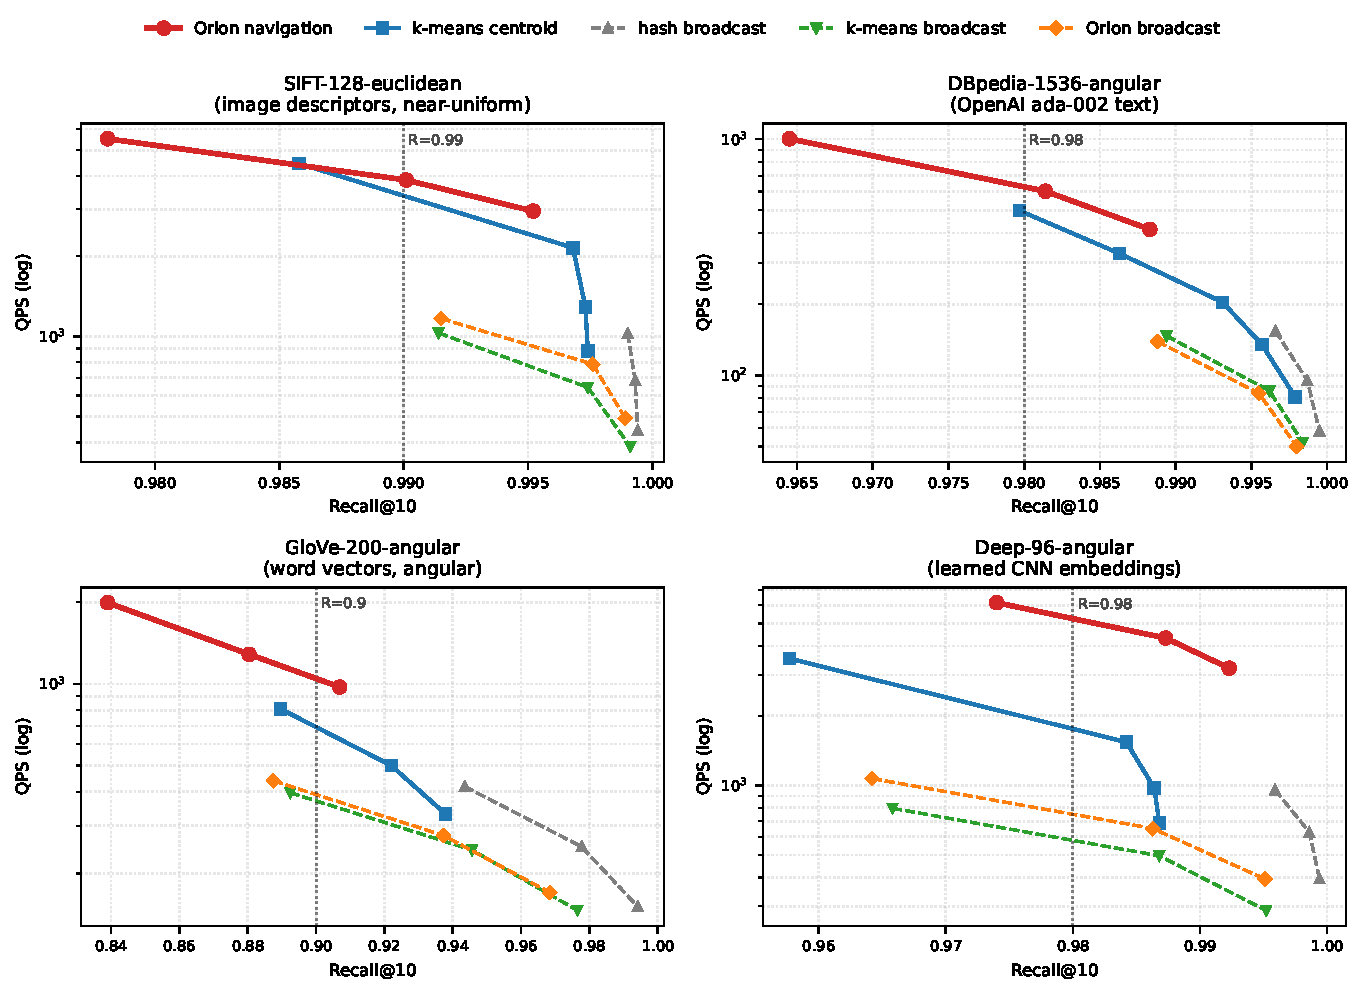
\includegraphics[width=\textwidth]{figures/frontiers.pdf}
\caption{Matched-recall throughput frontiers (QPS vs.\ Recall@10, log-$y$) for
the five serving arms on the four datasets, ordered by increasing geometric
difficulty. Orion navigation (red) dominates the upper-right of every panel; the
three broadcast arms (dashed) sit far below. The gap between Orion navigation and
$K$-means centroid (blue) is negligible on near-uniform SIFT and widens
monotonically to a $3.45\times$ throughput advantage on learned CNN embeddings.
Dotted vertical lines mark the operating point at which Table~\ref{tab:eval-qps}
reports QPS.}
\label{fig:frontiers}
\end{figure*}

\paragraph{Fan-out is the first-order lever.}
On all four datasets, every arm that reduces fan-out beats every broadcast arm by
$2.5\text{--}9\times$ at matched recall (Fig.~\ref{fig:frontiers}, dashed vs.\
solid; Table~\ref{tab:eval-qps}). Probing $\sim\!6/46$ (Deep), $\sim\!10/46$
(SIFT), $\sim\!14/46$ (DBpedia) or $\sim\!27/46$ (GloVe) shards is far cheaper
than probing all $46$, because a graph index's per-shard cost is
$\Theta(\log|\text{shard}|)$ and aggregate work scales with fan-out. This is
Orion's core, data-independent benefit and confirms fan-out as the objective
of~\eqref{eq:objective}. That the broadcast arms differ little among themselves
(hash vs.\ $K$-means vs.\ Orion layout) shows the win is the \emph{router}, not
the layout alone: locality is worthless unless a router exploits it.

\paragraph{Topology-aware routing tracks geometric difficulty.}
Table~\ref{tab:eval-qps} reads QPS at each dataset's operating point. Orion
navigation's advantage over the strongest simple router ($K$-means centroid)
grows exactly as the embedding's neighbor structure departs from smooth geometric
clusters: a statistical tie ($1.08\times$) on near-uniform SIFT, $1.30\times$ on
production OpenAI text embeddings (rising to $1.44\times$ at Recall $0.988$),
$1.49\times$ on GloVe, and $3.45\times$ on Deep---where the centroid router
cannot reach Recall $0.99$ at \emph{any} fan-out while Orion does so at fan-out
$\sim\!8$. This is the search-induced-topology hypothesis in action: on complex
manifolds the navigation graph, which follows the same structure the index was
built on, locates a query's neighbors in a handful of shards that nearest-centroid
routing spreads across many. Because every arm is single-copy, the advantage holds
at \emph{equal storage} and is not an artifact of replication.

\begin{table}[t]
\centering
\small
\begin{tabular}{@{}lrrrr@{}}
\toprule
& SIFT & DBpedia & GloVe & Deep \\
Arm & @0.99 & @0.98 & @0.90 & @0.98 \\
\midrule
Orion navigation   & \textbf{3874} & \textbf{636} & \textbf{1055} & \textbf{5333} \\
$K$-means centroid & 3576 & 490 & 710 & 1547 \\
hash broadcast     & 1025 & 154 & 418 & $\ge$956 \\
$K$-means broadcast& 1030 & 147 & 375 & 593 \\
Orion broadcast    & 1167 & 139 & 398 & 769 \\
\midrule
nav\,/\,centroid   & $1.08\times$ & $1.30\times$ & $1.49\times$ & $3.45\times$ \\
\bottomrule
\end{tabular}
\caption{QPS at the matched-recall operating point of Fig.~\ref{fig:frontiers}
(dotted lines), for the five arms on the four datasets. The last row is Orion
navigation's advantage over $K$-means centroid, which grows monotonically with
geometric difficulty (left to right). Deep is $10$M points and DBpedia is
$1536$-d, so absolute QPS is comparable only \emph{within} a column.}
\label{tab:eval-qps}
\end{table}

\paragraph{Threats to validity.}
The testbed is a single host with loopback transport, so absolute QPS and the
$46$-shards-on-$4$-peers packing are not portable; only within-dataset cross-arm
ratios are. Co-tenant interference keeps the strict host-quiet gate from passing
($6\text{--}13\%$), but every arm sees the same host and the reported ratios far
exceed the noise. At $1536$ dimensions the coordinator's $46$-way
scatter-gather/merge is a larger share of each query, lowering server saturation
on DBpedia ($70\text{--}78\%$) and making its absolute QPS coordinator-influenced;
the cross-arm ratios (same coordinator for every arm) are unaffected. Physical
multi-machine scale-out and the $P$-sweep correlation of the offline
navigation-weighted cut with realized fan-out (Lemma~\ref{lem:fanout}) are
out of scope for this single-host study.

% ------------------------- STANDALONE (uncomment) --------------------------
% \end{document}
% ---------------------------------------------------------------------------
